\documentclass[main.tex]{subfiles}
% 标架与参考系
\begin{document}


经典力学中的观察者对时间的感受依赖他所观察到的物理事件发生的先后顺序。以下我们通过物理事件的概念引出时间的概念,请结合图\ref{fig:III.5.1}进行理解。

\begin{figure}[ht]
    \centering
    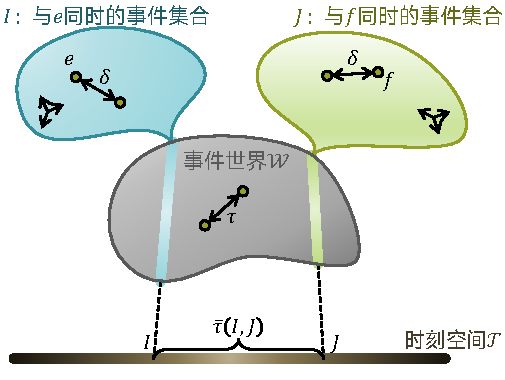
\includegraphics[width=0.5\textwidth]{images/III.5.1.pdf}
    \caption{事件世界概念示意图。图中字母符号与文中相同。}
    \label{fig:III.5.1}
\end{figure}

$\emph{事件世界(event-world)}\pazocal{W}$是一个非空集合,其元素$e\in\pazocal{W}$称为一个\emph{事件(event)}。$\pazocal{W}$上还定义一个\emph{时延函数}$\tau:\pazocal{W}^2\rightarrow\mathbb{R}$,满足:
\begin{description}
    \item[T1] $\forall e,f\in\pazocal{W},\quad\tau\left(e,f\right)=-\tau\left(f,e\right)$
    \item[T2] $\forall e,f,g\in\pazocal{W},\quad\tau\left(e,f\right)+\tau\left(f,g\right)=\tau\left(e,g\right)$
    \item[T3] $\forall e\in\pazocal{W}\forall t\in\mathbb{R}\exists f\in\pazocal{W},\quad\tau\left(e,f\right)=t$
\end{description}

所谓“事件”或“物理事件”是物理观测经验事实的“最小单元”。一个事件需且仅需用时间中的一个时刻和空间中的一个点来表示,在经典条件下可理解为“某物质点在某时刻出现在空间某处”。时延函数的定义规定了任意两个事件的时间间隔取值是一个实数。实数域$\mathbb{R}$具有\emph{完备性(completeness)},即在任意两个不相等的实数间必有一个实数。把时延函数的值域定为实数,使得我们可以考虑“随时间连续发生的一系列事件”,比如一个质点的运动轨迹。在时延函数的3个规定中,T1和T2的规定是符合直觉的,而T3的意思是,事件世界的元素在时延函数作用下具有封闭性。即无论从哪个事件开始算起,任意时延后都允许有一个事件的发生。这相当于说,事件世界包括了\emph{所有可发生的事件}。

我们还能说:
\begin{itemize}
    \item 事件$a$早于事件$b$,当且仅当$\tau\left(a,b\right)>0$;
    \item 事件$a$晚于事件$b$,当且仅当$\tau\left(a,b\right)<0$;
    \item 事件$a$与$b$\emph{同时(simultaneous)}发生,当且仅当$\tau\left(a,b\right)=0$;
\end{itemize}

事件的\emph{同时性(simultaneity)}形成了一个等价关系
\[S\equiv\left\{\left(a,b\right)\in\pazocal{W}^2|\tau\left(a,b\right)=0\right\}\]
我们称$S$是物理事件的同时关系。由等价关系的基本定理\ref{thm:II.1.1},通过$S$可对事件世界$\pazocal{W}$形成划分$\pazocal{T}\equiv\pazocal{W}\setminus S$,使得对任一$e\in\pazocal{W}$,$I\equiv\left\llbracket e\right\rrbracket_S\in\pazocal{T}$是事件$e$关于同时关系$S$的等价类。我们称$\pazocal{T}$为\emph{时刻空间(instant space)}。时刻空间的元素$I,J,\cdots\in\pazocal{T}$称为\emph{时刻(instants)},它们是不同时刻下同时发生的所有事件的集合。

设$I,J\in\pazocal{T}$是两个时刻,我们可以通过$I$和$J$的任一元素$e\in I$和$f\in J$来表示这两个时刻的间隔。具体地,定义在$\pazocal{T}$上的函数$\overline{\tau}:\pazocal{T}^2\rightarrow\mathbb{R}$,
\[\overline{\tau}\left(I,J\right)=\tau\left(e,f\right),\quad\forall e\in I\forall f\in J\]
的结果就是时刻$I$、$J$的时间间隔。我们可以设计符合我们以往习惯的记法:$\forall I,J\in\pazocal{T},$
\[I-J\equiv\overline{\tau}\left(I,J\right)\]
若$s=\overline{\tau}\left(I,J\right)$,则又可记$I=J+s$。注意,我们没有定义两个时刻的“和”($I+J$)的意义。事实上,时刻空间$\pazocal{T}$与实数集$\mathbb{R}$是自然同构的。因此在进行时刻之间的运算时,我们可以默认$\pazocal{T}$就像$\mathbb{R}$。但是每一$\pazocal{T}$中的时刻又是同时事件构成的欧几里得空间,这时$\pazocal{T}$比实数集$\mathbb{R}$具有更多含义,故我们仍保持提及$\pazocal{T}$。

接下来,我们定义两个同时发生的事件之间的距离。\emph{距离函数}是定义在$S$上的映射$\delta:S\rightarrow\mathbb{R}$,满足:
\begin{description}
    \item[D1] 对任一时刻$I\in\pazocal{T}$,$\delta$在$I^2\subset S$上的限制$\left.\delta\right|_{I^2}$使作为事件集合的$I$成为一个以事件为点的欧几里得空间,其平称空间记为$\mathcal{V}_I$;
    \item[D2] $\dim\mathcal{V}_I=3,\quad\forall I\in\pazocal{T}$。
\end{description}

距离函数$\delta$定度在同时关系$S$上,说明只有同时发生的事件之间才能讨论距离。$S$中含有不同时刻下的同时事件,所以在不同时刻下,我们都用同一度量$\delta$来测定距离。规定D1用通俗语言说就是每一时刻$I$作为同时事件的集合,在用了度量$\delta$之后,能够形成欧几里得空间,即能够满足定义\ref{def:II.3.4}。结合规定D2,每一时刻下的欧几里得空间都是3维的。

规定T1\textasciitilde T3、D1\textasciitilde D2共同形成了新经典时空的概念。正式陈述如下——

\begin{definition}[新经典时空]\label{def:III.5.1}
    若集合$\pazocal{W}$具有T1\textasciitilde T3规定的时延函数和D1\textasciitilde D2规定的距离函数,则称$\pazocal{W}$是\emph{新经典时空(neo-classical spacetime)}。
\end{definition}

我们可以形象地把时延函数和距离函数理解为观察者所使用的时钟和直尺。在新经典时空的定义下,没有钟慢效应,因为“同时性”的定义是绝对的;也没有尺缩效应,因为距离函数的定义是绝对的。在这样的时空观下,本讲义介绍的连续介质力学基础适用的范围自然就是经典低速运动和形变。

事件世界$\pazocal{W}$上的自同态映射$\alpha:\pazocal{W}\rightarrow\pazocal{W}$应满足
\begin{align*}
    \tau\left(\alpha\left(e\right),\alpha\left(f\right)\right)   & =\tau\left(e,f\right),\quad\forall e,f\in\pazocal{W} \\
    \delta\left(\alpha\left(e\right),\alpha\left(f\right)\right) & =\delta\left(e,f\right),\quad\forall e,f\in S
\end{align*}
其中$S$是$\pazocal{W}$上的同时关系。事实上映射$\alpha$就是对其所作用的事件进行了一个时移。若记$U^\alpha$为$\pazocal{W}$上的自同态映射$\alpha$在$\pazocal{W}$的子集$U$上的限制的像集,即$U^\alpha\equiv\mathrm{ran}\left.\alpha\right|_U$,则易验
\[\overline{\tau}\left(I^\alpha,J^\alpha\right)=\overline\tau\left(I,J\right),\quad\forall I,J\in\pazocal{T}\]
或按之前规定的记法:
\[J^\alpha-I^\alpha=J-I,\quad\forall I,J\in\pazocal{T}\]其中$\pazocal{T}$是$\pazocal{W}$上的时刻空间。上式等号两边同时加上$I^\alpha-J$得
\[I^\alpha-I=J^\alpha-J,\quad\forall I,J\in\pazocal{T}\]
也就是说,映射$\alpha$对不同时刻下的事件进行作用前后的时间间隔是只依赖$\alpha$的固定值。因此可记由任一时刻$I$及其对应的$I^\alpha$规定的实数$s_\alpha\equiv I^\alpha-I,\forall I\in\pazocal{T}$为由$\alpha$引出的\emph{时移(time-shift)}。由规定T3可以证明,对应于每一个$\pazocal{W}$上的自同态映射$\alpha$有且只有一个实数$s_\alpha\in\mathbb{R}$满足$s_\alpha=I^\alpha-I$。留意到一个时刻$I$同时又是一个欧几里得空间,对任一时刻$I$,$\alpha$是$I$到$I^\alpha$关于共同的度量$\delta$的保距映射,故上述论断亦表明$\alpha$是一个等距变换(双射)。相应地也可证明,对应于每一$\pazocal{W}$上的自同态映射$\alpha$有且只有一个由$I$的平移空间$\mathcal{V}_I$到$I^\alpha$的平移空间$\mathcal{V}_{I^\alpha}$的同态映射(即线性变换)$\mathbf{A}_I:\mathcal{V}_{I}\rightarrow\mathcal{V}_{I+s_\alpha}$满足$\mathbf{A}_I\left(f-e\right)=\alpha\left(f\right)-\alpha\left(e\right),\forall e,f\in I$。
\end{document}